\chapter{Pricipais Conceitos e Trabalhos Relacionados}\label{cap_2}

\section{Aprendizado de Máquina}

Um algoritmo de \ac{ML} é capaz de aprender a partir de dados, aperfeiçoando seu desempenho por meio da experiência acumulada \cite{goodfellow2016deep}. De forma complementar, \citeonline{mitchell1997ml} estabelece que: ``um programa de computador é dito aprender a partir de uma experiência E, em relação a uma classe de tarefas T e uma medida de desempenho P, se seu desempenho em T, conforme mensurado por P, melhora com a experiência E''.


%\subsection{Tarefas}

O aprendizado de máquina organiza suas tarefas a partir da forma como o sistema deve processar os dados de entrada, denominados exemplos. Um exemplo consiste em um conjunto de características quantitativamente mensuradas de um objeto ou evento de interesse. Tipicamente, representa-se um exemplo como um vetor $\mathbf{x} \in \mathbb{R}^n$, em que cada componente $x_i$ corresponde a uma característica do objeto analisado \cite{goodfellow2016deep}.

Entre os tipos de tarefas mais recorrentes no contexto de \ac{ML}, destacam-se: regressão, transcrição, tradução automática, classificação, detecção de anomalias, síntese de amostragem, segmentação semântica. 

%\begin{itemize}

%\item regressão: a previsão de um valor contínuo a partir de entradas específicas.

%\item Transcrição: dados não estruturados são convertidos em forma textual, reconhecimento óptico e no reconhecimento de fala.

%\item Tradução automática: conversão de sequências de símbolos de uma linguagem para outra.

%\item Classificação: dado um valor de entrada, seja texto ou imagem, o algoritmo devolve a classificação da entrada em determinada classe.

%\item Detecção de anomalias: identifica eventos atípicos.

%\item Síntese de amostragem: novos exemplos similares aos dados originais são gerados.

%\end{itemize}


\subsection{Segmentação Semântica}

A segmentação semântica consiste na tarefa de atribuir, a cada pixel de uma imagem, um rótulo que representa a classe semântica à qual aquele pixel pertence \cite{casanova2020reinforced}. Diferentemente de tarefas como classificação ou detecção, a segmentação não apenas prediz a categoria presente na imagem, mas também preserva a estrutura espacial das regiões segmentadas, fornecendo um mapeamento denso das classes no domínio da imagem \cite{cheng2023survey_segmentation}.

Essa capacidade de produzir uma representação espacialmente coerente torna a segmentação semântica um componente central em diversos sistemas avançados. A partir das máscaras geradas, é possível derivar tarefas complementares, como localização e contagem de objetos, estimativa de forma, análise morfológica e detecção de anomalias estruturais.

Nos últimos anos, sua utilização tem crescido substancialmente em aplicações críticas, incluindo análise de imagens médicas, direção autônoma, realidade aumentada, vigilância e reconstrução tridimensional, consolidando-a como uma ferramenta essencial em ambientes que demandam compreensão visual precisa e contextualizada \cite{cheng2023survey_segmentation}.

A Figura \ref{fig:segmentation} ilustra o processo de segmentação realizado pelos modelos propostos, destacando a natureza da tarefa de segmentação semântica. Inicialmente, tem-se a imagem original de entrada e o respectivo ground-truth, referente à anotação de referência em nível de pixel, na qual cada elemento da imagem recebe o rótulo da classe a que pertence (Figuras \ref{fig:segmentation}a e \ref{fig:segmentation}b, respectivamente). Após a predição realizada pelo modelo (Figura \ref{fig:segmentation}c), a qualidade da segmentação é estimada por meio da comparação direta e quantitativa entre a predição e o groudn-truth, utilizando, entre outras, a métrica \ac{IoU}.

%\textcolor{red}{A Figura \ref{fig:segmentation} ilustra o processo de segmentação realizado pelos modelos propostos, destacando a natureza da tarefa de Segmentação Semântica. O painel em (a) exibe a imagem original de entrada. O painel (b) apresenta o Ground-Truth, que corresponde à anotação de referência pixel a pixel, onde cada pixel recebe o rótulo da classe real à qual pertence. O painel (c) mostra a Predição do Modelo, que é o resultado da inferência da rede neural. A qualidade da segmentação é avaliada pela comparação direta e quantitativa entre a Predição e o Ground-Truth, utilizando métricas como o \ac{IoU}.}




\begin{figure}[h!]
\centering
\caption{Exemplo ilustrativo de segmentação semântica. (a) imagem original contendo três classes de objetos (gato, cachorro e planta). (b) imagem com as máscaras de segmentação (ground-truth) discriminadas por classe. (c) imagem resultante da segmentação por classe.}
%\caption{\textcolor{red}{Exemplo de segmentação semântica. Em (a) temos três classes (Gato, Cachorro e Planta). A imagem (b) representa a máscara de segmentação separada por classe. Em (c) temos o retorno da imagem segmentada por classe.}}
\begin{tabular}{ccc}
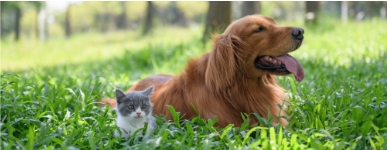
\includegraphics[height=2cm]{Segmentation.png} & 
\includegraphics[height=2cm]{Segmentation-b.png} &
\includegraphics[height=2cm]{Segmentation-c.png}\\
(a) & (b) & (c)
\end{tabular}
\label{fig:segmentation}
{\small Fonte: \cite{minaee2020survey}}
\end{figure}


%\begin{figure}[h!]
%\centering
%\caption{\textcolor{red}{Exemplo de segmentação semântica. Em (a) temos três classes (Gato, Cachorro e Planta). A imagem (b) representa a máscara de segmentação separada por classe. Em (c) temos o retorno da imagem segmentada por classe.}}
%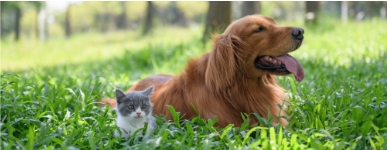
\includegraphics[width=1\textwidth]{Segmentation.png}
%\label{fig:segmentation}
%{\small Fonte:  \cite{minaee2020survey}}
%\end{figure}


\subsection{Classificação dos Algoritmos de Aprendizado de Máquina}

O algoritmo de aprendizado de máquina pode ser classificado em diferentes paradigmas de treinamento, dos quais se destacam o aprendizado supervisionado, não supervisionado, semi-supervisionado, por reforço e ativo.

No aprendizado supervisionado, o modelo recebe um conjunto de exemplos rotulados como dados de treinamento e aprende uma função que mapeia entradas para saídas desejadas. Após o treinamento, o modelo é capaz de realizar predições sobre exemplos não observados previamente. Este paradigma é amplamente uitilizado em tarefas como classificação, regressão e ranqueamento.

No aprendizado não supervisionado, o modelo tem acesso apenas a exemplos não rotulados e objetiva identificar estruturas, padrões latentes ou agrupamentos naturais presentes nos dados. Nesse contexto, a ausência de rótulos torna a avaliação quantitativa mais desafiadora. Problemas típicos incluem agrupamento (clustering), detecção de padrões, modelagem de densidade e redução de dimensionalidade.

No aprendizado semi-supervisionado, o modelo recebe um conjunto de treinamento composto simultaneamente por exemplos rotulados e não rotulados. Essa abordagem é adequada em cenários nos quais grandes volumes de dados não rotulados estão disponíveis, enquanto a rotulagem manual é custosa ou demorada. Tarefas como classificação, regressão e ranqueamento podem ser formuladas sob este paradigma. Assumindo que os dados não rotulados sigam a mesma distribuição que os dados rotulados, espera-se que sua exploração contribua para melhorar o desempenho em relação ao aprendizado supervisionado puro.

O Aprendizado por Reforço (\ac{RL}) constitui um subcampo da Inteligência Artificial (\ac{AI}) no qual um agente aprende a tomar decisões por meio da interação contínua com um ambiente, aprimorando progressivamente sua política de ação com base no feedback recebido \cite{ghasemi2024comprehensive}. Esse paradigma é inspirado nos mecanismos de aprendizado por tentativa e erro observados em humanos e animais, nos quais a exploração do ambiente desempenha um papel fundamental na aquisição de conhecimento, sem a necessidade de supervisão explícita \cite{li2022xrl}.
%O trecho a seguir apresenta, de forma concisa, a formulação clássica de \ac{RL}:

Um agente de aprendizado por reforço interage com um ambiente ao longo do tempo. A cada instante $t$, o agente observa um estado $s_t$ pertencente ao espaço de estados $\mathcal{S}$ ($s_t \in \mathcal{S}$) e seleciona uma ação $a_t$ do espaço de ações $\mathcal{A}$ ($a_t \in \mathcal{A}$), seguindo uma política \( \pi(a_t|s_t) \), responsável por mapear estados ($s_t$) em ações ($a_t$), representando o comportamento do agente. Após a execução de $a_t$, o agente recebe uma recompensa escalar $r_t$ e transita para o estado subsequente $s_{t+1}$, de acordo com a dinâmica do ambiente (ou modelo). Essa dinâmica é descrita pela função de recompensa R(s,a) e pela probabilidade de transição $P(s_{t+1}\|s_t, a_t)$.
Em problemas episódicos, a interação prossegue até que um estado terminal seja alcançado e o episódio seja reiniciado. O retorno
\( R_t = \sum_{k=0}^{\infty} \gamma^k r_{t+k} \)
%$R_t$ = $\sum_{k=0}^{\infty}$ $\gamma^k$ $r_{t+k}$
é definido como a soma acumulada das recompensas descontadas, em que $\gamma \in (0,1]$ representa o fator de desconto. O objetivo do agente é maximizar a expectativa desse retorno de longo prazo a partir de cada estado.

Uma formulação matemática central que sustenta o \ac{RL} é o Processo de Decisão de Markov (\ac{MDP}), que modela problemas de tomada de decisão sequencial nos quais a transição entre estados depende apenas do estado atual e da ação executada \cite{li2022xrl}. Formalmente, um \ac{MDP} é definido como um quíntuplo (S, A, P, R, $\gamma$), em que S é o conjunto de estados possíveis; A é o conjunto de ações disponíveis; P é a função de transição de estados; R é a função de recompensa; $\gamma$ é o fator de desconto.

O objetivo do agente é encontrar uma política ótima que maximize a recompensa acumulada esperada, denominada retorno $G_t$. Para tal, utilizam-se tipicamente duas funções de valor: a função de valor de estado $V(s)$, que estima o retorno esperado a partir do estado $s$, e a função de valor estado-ação $Q(s,a)$, que estima o retorno esperado a partir do estado $s$ quando tomada a ação $a$ \cite{ghasemi2024comprehensive}.


%\begin{quote}

%\textbf{Aprendizado supervisionado:} O aprendiz recebe um conjunto de exemplos rotulados como dados de treinamento e realiza predições para todos os pontos não observados. Este é o cenário mais comum, associado a problemas de classificação, regressão e ranqueamento. O problema de detecção de spam, discutido na seção anterior, é um exemplo típico de aprendizado supervisionado.

%\textbf{Aprendizado não supervisionado:} O aprendiz recebe exclusivamente dados de treinamento não rotulados e realiza predições para pontos não vistos. Como, geralmente, não há exemplos rotulados disponíveis neste cenário, torna-se difícil avaliar quantitativamente o desempenho do aprendiz. Exemplos típicos de aprendizado não supervisionado incluem problemas de agrupamento (clustering) e redução de dimensionalidade.

%\textbf{Aprendizado semi-supervisionado:} O aprendiz recebe um conjunto de treinamento composto por dados rotulados e não rotulados, e realiza predições para pontos não observados. Essa abordagem é comum em contextos nos quais dados não rotulados são facilmente acessíveis, mas a rotulagem é cara ou trabalhosa. Diversos tipos de problemas, incluindo classificação, regressão e ranqueamento, podem ser enquadrados nesse paradigma. Espera-se que a distribuição dos dados não rotulados acessíveis possa auxiliar o aprendiz a alcançar um desempenho superior ao do aprendizado supervisionado puro.

%\end{quote}

%\begin{flushright}
%\footnotesize \cite{mohri2018foundations}
%\end{flushright}

\subsubsection{Aprendizado Ativo}

Diversas técnicas de \ac{ML} requerem grandes conjuntos de dados de treinamento para atingir seu desempenho ideal. Entretanto, o processo de anotação é frequentemente custoso, demorado e exige mão de obra especializada \cite{konyushkova2017learning}. 
No paradigma supervisionado, o algoritmo recebe um conjunto S composto por exemplos rotulados por especialistas, o que, em tarefas como segmentação de imagem, pode demandar horas de trabalho manual para rotular pixel a pixel. A partir desse conjunto, o modelo aprende uma função que mapeia os dados de entrada para as saídas desejadas.

%Para o processo de aprendizado de máquina supervisionado, o algoritmo recebe um dado $S$, rotulado por um especialista, muitas vezes demandando horas para que todos os pixels sejam rotulados. Ao receber esse conjunto de dados rotulado, o modelo aprenderá uma função que mapeia as entradas e produza a saída desejada. 

Durante o treinamento, o modelo processa pares $x_i,y_i$, em que $x_i$ representa a imagem original e $y_i$ a saída esperada.
Contudo, a exigência de um conjunto $S$ completamente rotulado torna o processo oneroso e pouco escalável. Nesse contexto, o aprendizado ativo \ac{AL} propõe estratégias para reduzir o custo de anotação por meio da seleção das amostras mais informativas para o treinamento \cite{settles2009active}. Dessa forma, em vez de rotular todo o conjunto de dados, o sistema seleciona iterativamente apenas os exemplos que proporcionam maior ganho esperado de desempenho, reduzindo substancialmente o esforço de anotação humana.

%Todavia, é necessário, durante esse processo, que haja um dado $S$ rotulado. Para reduzir o custo e o esforço envovlido na rotulagem, o Active Learning \ac{AL} propõe estratégias que selecionam os exemplos mais informativos e produtivos para anotação, otimizando o processo de treinamento e o custo para aquisição de modelos inteiramente rotulados \cite{settles2009active}.

\begin{figure}[h!]
\centering
\caption{Processo de funcionamento do ciclo de aprendizado ativo tradicional, destacando as etapas de treinamento inicial, seleção de amostras informativas, anotação pelo especialista e atualização incremental do modelo.}
%\caption{Processo de funcionamento do ciclo de aprendizado do modelo de Aprendizado Ativo}
\includegraphics[width=10cm]{Active_Learning.png}
\label{fig:active_learning}\\
{\small Fonte: \cite{saito2014active}}
\end{figure}


De acordo com \citeonline{casanova2020reinforced}, os métodos de aprendizado ativo podem ser categorizados em dois grandes grupos: métodos baseados em estratégias projetadas manualmente e métodos orientados por dados.
Métodos baseados em estratégias projetadas manualmente agrupam abordagens que combinam heurísticas clássicas como incerteza, diversidade e representatividade \cite{konyushkova2017learning, bachman2017learning, konyushkova2018discovering, woodward2017active}. Já em métodos orientados por dados, o próprio modelo aprende quais amostras são mais informativas, utilizando o histórico de treinamento e estimadores internos de qualidade/amostragem \cite{konyushkova2017learning, bachman2017learning, konyushkova2018discovering, woodward2017active}.

A Tabela \ref{tab:active_learning_strategies} sintetiza e compara as principais estratégias de aprendizado ativo presentes na literatura. Nota-se que métodos guiados por incerteza, como a entropia, destacam-se no contexto de segmentação semântica, já que a maior concentração de incerteza ocorre tipicamente nas bordas dos objetos, regiões críticas que demandam maior atenção durante a correção manual dos rótulos.

%\textcolor{red}{A Tabela \ref{tab:active_learning_strategies} cria um comparativo entre as principais abordagens utilizadas.} 

%\textcolor{red}{Segundo a tabela \ref{tab:active_learning_strategies}, as abordagens baseadas em Incerteza (como a Entropia) são particularmente vantajosas para a segmentação semântica, pois a 'dúvida' do modelo geralmente se concentra nas bordas dos objetos, que é exatamente onde o refinamento humano é mais necessário.}


\begin{table}[h!]
\centering
\caption{Comparativo das principais estratégias de Active Learning.}
\label{tab:active_learning_strategies}
\resizebox{\textwidth}{!}{
\begin{tabular}{|p{2.5cm}|p{4.5cm}|p{4.5cm}|p{4.5cm}|p{3.5cm}|}
\hline
\textbf{Estratégia} & \textbf{Princípio de Seleção} & \textbf{Vantagens} & \textbf{Limitações} & \textbf{Exemplos}\\
\hline
\hline
\textbf{Baseada em Incerteza}\newline (Uncertainty-based) & 
Seleciona amostras com maior incerteza do modelo (alta entropia) & %em que o modelo tem a menor confiança na predição (maior entropia) & 
- Fácil de implementar\newline - Eficaz para refinar fronteiras de decisão (bordas na segmentação) & 
- Pode priorizar ruídos ou outliers\newline - Baixa diversidade das amostras selecionadas & 
- \ac{LC}\newline - \ac{ES}\newline - MC Dropout\\
\hline
\textbf{Baseada em Diversidade}\newline (Diversity-based) & 
Seleciona amostras que melhor representam a distribuição dos dados não rotulados & % (espalhamento) & 
- Reduz redundância\newline - Favorece cobertura de casos raros & %Evita redundância nos dados\newline - Garante cobertura de casos raros no conjunto de dados & 
- Alto custo computacional (clustering, distâncias no espaço latente) & %Custo computacional elevado (requer clustering ou cálculo de distâncias em todo o pool) & 
- Coreset\newline - $k$-Center-Greedy\newline - Clustering\\
\hline
\textbf{Mudança Esperada no Modelo}\newline \ac{EMC} & 
Seleciona amostras que potencialmente causariam maior impacto nos gradientes/perda & %Seleciona amostras que causariam a maior alteração nos gradientes ou na perda do modelo se fossem rotuladas & 
- Teoricamente a mais robusta, pois foca na melhoria direta do treino & 
- Muito lenta para \ac{DL} (exige simulações de treino) & %Extremamente lenta para Deep Learning (exige retreinos simulados ou cálculos pesados de gradiente) & 
- \ac{EGL}\\
\hline
\textbf{Híbrida}\newline (Hybrid) & 
Combina incerteza e diversidade para balancear informação e representatividade & %selecionar amostras informativas e representativas & 
- Equilibra exploration (diversidade) e exploitation (incerteza)\newline - Estado da arte atual & %Balanceia a exploração (diversidade) e a explotação (incerteza)\newline - Estado da arte atual & 
- Mais complexa de configurar (pesos e critérios combinados) & %Mais complexa de ajustar (hiperparâmetros de peso entre incerteza e diversidade) & 
- \ac{BADGE}\newline - \ac{VAAL}\\
\hline
\end{tabular}%
}
\fonte{Adaptado de \citeonline{ren2021survey}}
\end{table}



%\begin{itemize}
%\item Métodos que combinam diferentes estratégias de AL projetadas manualmentes (Roy \& McCallum, 2001; Osugi et al., 2005; Gal et al., 2017; Baram et al., 2004;
%Chu \& Lin, 2016; Hsu \& Lin, 2015; Ebert et al., 2012; Long \& Hua, 2015)

%\item Abordagens de AL orientadas por dados (Bachman et al., 2017; Fang et al., 2017; Konyushkova et al., 2017; Woodward \& Finn, 2016; Ravi \& Larochelle, 2018; Konyushkova et al., 2018) aprendem quais amostras são mais informativas para treinar um modelo usando informações do próprio modelo.
%\end{itemize}


%\subsubsection{Aprendizado por Reforço}

%Aprendizado por Reforço (Reinforcement Learning (\ac{RL})) é um subcampo da Inteligência Artificial (\ac{AI}), na qual um agente aprende a tomar decisões interagindo com o ambiente, potencializando a melhora do algoritmo de aprendizado \cite{ghasemi2024comprehensive}.

%Esse paradigma é inspirado nos mecanismos de aprendizado de tentativa e erro de humanos, onde o envolvimento com o ambiente serve como uma abordagem fundamental pra aprendizado sem um guia externo \cite{li2022xrl}.

%O trecho a seguir descreve formalmente como é o funcionamento do \ac{RL}.

%\begin{quote}
%Um agente de aprendizado por reforço (RL) interage com um ambiente ao longo do tempo. A cada instante de tempo \( t \), o agente recebe um estado \( s_t \) pertencente ao espaço de estados \( \mathcal{S} \), e seleciona uma ação \( a_t \) do espaço de ações \( \mathcal{A} \), seguindo uma política \( \pi(a_t|s_t) \), que representa o comportamento do agente, isto é, um mapeamento de estados \( s_t \) para ações \( a_t \).

%Em seguida, o agente recebe uma recompensa escalar \( r_t \) e transita para o próximo estado \( s_{t+1} \), de acordo com a dinâmica do ambiente (ou modelo), que é descrita pela função de recompensa \( R(s, a) \) e pela probabilidade de transição de estado \( P(s_{t+1}|s_t, a_t) \), respectivamente.

%Em problemas episódicos, esse processo continua até que o agente alcance um estado terminal, após o qual o episódio reinicia.

%O retorno \( R_t = \sum_{k=0}^{\infty} \gamma^k r_{t+k} \) é a soma acumulada das recompensas descontadas, onde \( \gamma \in (0, 1] \) é o fator de desconto.

%O objetivo do agente é maximizar a expectativa desse retorno de longo prazo a partir de cada estado.

%\end{quote}

%\begin{flushright}
%\footnotesize \cite{li2017drl}
%\end{flushright}

%Um dos paradigmas considerados um problema é como um agente interage com o ambiente para maximizar sua recompensa acumulada. A resposta pra esse problema é um processo conhecido como Processo de Decisão de Markov (\ac{MDP}) \cite{li2022xrl}

%O \ac{MDP} é um modelo de tomada de decisão sequencial no qual as transições de estado e recompensas dependem do estado atual e da ação tomada. Ele é formado um conjunto quíntuplo $(S, A, P, R, \gamma)$, onde:

%\begin{itemize}
%    \item $S$: Conjunto de estados
%    \item $A$: Conjunto de ações
%    \item $P$: Função de transição de estados
%    \item $R$: Função de recompensa
%    \item $\gamma$: Fator de desconto
%\end{itemize}

%O objetivo é encontrar uma política que maximize a recompensa acumulada esperada, chamada de retorno $G_t$. Para que isso ocorra, utiliza-se uma função $V_t(s)$, que estima o retorno esperado a partir do estado $s$, e $Q_a(s,a)$, que estima o retorno esperado a partir do estado $s$ quando tomada a ação $a$. \cite{ghasemi2024comprehensive}

\section{Superpixels}

Superpixels consistem na partição de uma imagem em regiões coesas formadas por pixels com características semelhantes, usualmente em termos de cor, textura e proximidade espacial, resultando em unidades elementares maiores e mais estruturadas do que pixels individuais. Essa representação reduz significativamente a redundância local e, por consequência, o volume de elementos a serem processados, o que contribui para acelerar etapas posteriores de segmentação e análise de imagens \cite{barcelos2024superpixel}. Nas últimas décadas, técnicas baseadas em superpixels têm recebido crescente atenção na literatura, especialmente devido ao seu potencial para reduzir o custo computacional e aumentar a eficiência em tarefas de segmentação semântica e instanciada \cite{vargas2014superpixel}.

A Figura \ref{fig:duas_figuras} ilustra um exemplo de imagem do conjunto de dados Cityscapes após etapas de processamento. Na Figura \ref{fig:duas_figuras}a, é apresentada a predição de segmentação semântica gerada pelo modelo \ac{SLIC}. Na Figura \ref{fig:duas_figuras}b tem-se a imagem particionada em unidades de superpixels adaptativos \cite{kim2023adaptive}, uma técnica de amostragem baseada em região (Region-Based Sampling) empregada no \ac{AL}. Nessa abordagem, os superpixels são utilizados como blocos elementares para identificar e selecionar regiões com maior incerteza preditiva (alta entropia), otimizando o processo de anotação ao direcionar o esforço humano apenas aos segmentos mais informativos para o treinamento subsequente. %Tal abordagem utiliza os superpixels como blocos elementares para calcular e amostrar regiões de maior incerteza preditiva (alta entropia), permitindo a otimização do processo de anotação ao focar o esforço humano apenas nos segmentos mais informativos para o treinamento subsequente.}

%Superpixel consiste em particionar imagens em regiões compostas por similiridade, criando pixels conectados. Isso ajuda a acelerar o processo de segmentação de imagem, reduzindo o trabalho que a máquina terá para processar informações redundantes  \cite{barcelos2024superpixel}
%Atualmente, superpixels tem recebido uma atenção especial para acelerar a segmentação de imagem \cite{vargas2014superpixel}.


\begin{figure}[h!]
\caption{Exemplo de imagens do conjunto de dados Cityscapes. (a)\textit{Ground-Truth} da imagem. (b) imagem particionada em superpixels}
\begin{tabular}{cc}
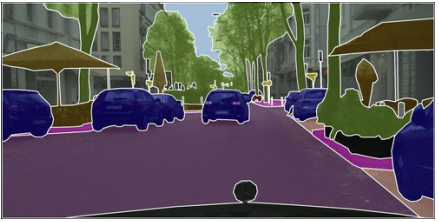
\includegraphics[height=3.75cm]{cap_comandos/figuras/Oracle_Superpixel.PNG} &
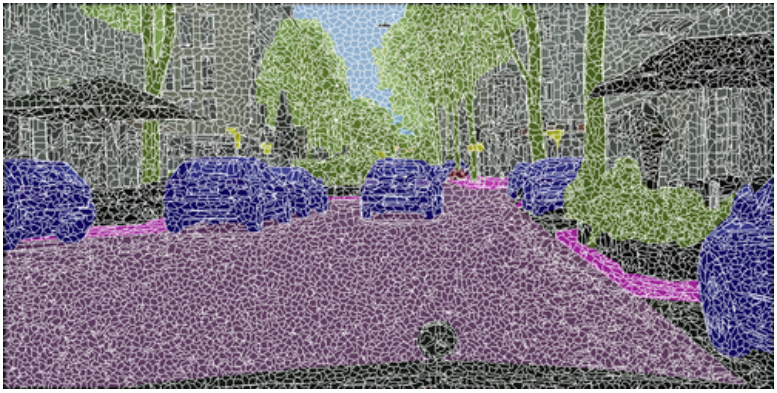
\includegraphics[height=3.75cm]{cap_comandos/figuras/SuperPixel.PNG}\\
(a) & (b)
\end{tabular}
\label{fig:duas_figuras}
\centering
{\small Fonte: \cite{kim2023adaptive}}
\end{figure}


%\begin{figure}[h!]
%\centering
%\caption{Divisão da imagem em superpixels}
%\begin{minipage}[b]{0.45\textwidth}
%\centering
%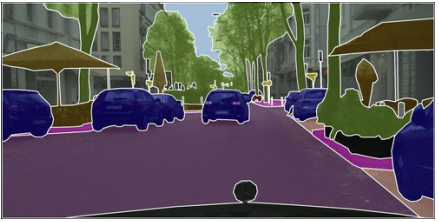
\includegraphics[width=\linewidth]{cap_comandos/figuras/Oracle_Superpixel.PNG}
%\caption*{Imagem segmentada original}
%\label{fig:figura1}
%\end{minipage}
%\hfill
%\begin{minipage}[b]{0.45\textwidth}
%\centering
%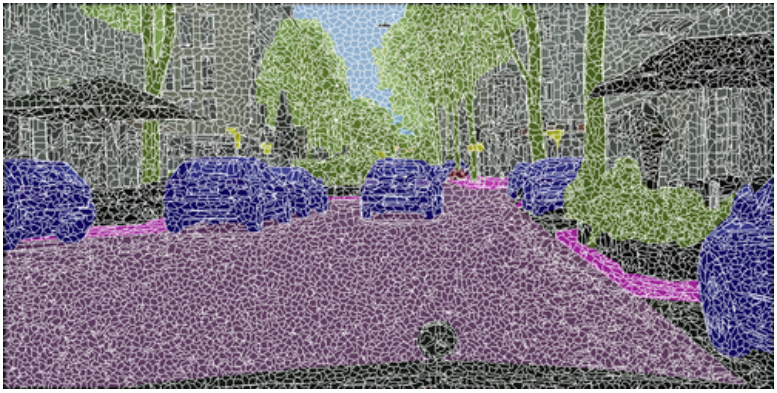
\includegraphics[width=\linewidth]{cap_comandos/figuras/SuperPixel.PNG}
%\caption*{Imagem com superpixels}
%\label{fig:figura2}
%\end{minipage}
%\label{fig:duas_figuras}

%\vspace{0.3em}
%\centering
%{\small Fonte: \cite{kim2023adaptive}}
%\end{figure}



\section{Interactive Learning}

O aprendizado interativo (\ac{IL}) consiste em um paradigma de treinamento no qual o usuário participa ativamente do processo de anotação ou correção, selecionando objetos de interesse de forma precisa e incremental por meio de entradas simples, tais como cliques, pontos, scribbles ou delimitações por caixa (\textit{bounding boxes}) \cite{xu2016deep_arxiv}.
A interação humana pode ser empregada tanto para orientar a segmentação de objetos específicos, quanto para refinar predições previamente geradas pelo modelo, corrigindo regiões mal segmentadas ou omitidas.

%O Aprendizado interativo (\ac{IL}) é o aprendizado que permite os usuários selecionarem os objetos de interesse precisavemente e interativamente provendo entradas como pontos ou seleções de caixa \cite{xu2016deep_arxiv}. 

O objetivo central da segmentação de imagens interativa é aproximar-se, com a maior fidelidade possível, da máscara de referência, utilizando o menor número de interações humanas, comumente mensuradas em número de cliques \cite{sofiiuk2020fbrs_arxiv}. Em geral, os sistemas oferecem uma interface na qual o usuário pode iterativamente adicionar cliques positivos e negativos até que o resultado atinja o nível de precisão desejado.
De modo geral, a literatura reporta duas direções complementares no uso de IL: (i) abordagens que empregam o sinal interativo como mecanismo de refinamento incremental do modelo de segmentação; e (ii) abordagens que utilizam a interação para guiar a segmentação de objetos específicos ou para corrigir inconsistências localizadas nas máscaras produzidas automaticamente.

A Figura \ref{fig:figura1} ilustra o fluxo de interação humano-computador no contexto da segmentação interativa. A imagem é apresentada ao usuário especialista por meio de uma interface gráfica, na qual ele fornece cliques de feedback para orientar o processo de refinamento. O botão esquerdo do mouse é utilizado para inserir \textit{foreground clicks} (pontos positivos), enquanto o botão direito registra \textit{background clicks} (pontos negativos), permitindo corrigir falhas na predição ou remover áreas indevidamente segmentadas. Esses cliques são interpretados pelo modelo como restrições rígidas (\textit{hard constraints}). Após cada iteração de processamento, o modelo retorna uma máscara de segmentação atualizada. Esse ciclo interativo se repete até que a segmentação atinja o nível de precisão desejado pelo especialista, caracterizando uma abordagem de aprendizado interativo (Interactive Learning).

%\textcolor{red}{A Figura \ref{fig:figura1} ilustra o fluxo de interação humano-computador no contexto da segmentação interativa. A imagem é apresentada ao usuário especialista por meio de uma interface gráfica para o fornecimento de cliques de feedback. O usuário utiliza o botão esquerdo para indicar os foreground clicks (pontos positivos) e o botão direito para fornecer os background clicks (pontos negativos), corrigindo falhas na predição ou áreas indesejadas. Esses inputs são interpretados pelo modelo como restrições (hard constraints). Após o processamento, o modelo retorna a máscara de segmentação refinada. O ciclo de refinamento iterativo é repetido até que a segmentação atinja a precisão desejada pelo especialista, caracterizando uma abordagem de aprendizado interativo (Interactive Learning).}

%A seleção de objetos de interesse através de demarcações utilizando especialistas pode ser utilizada tanto para a segmentação de objetos específicos, quanto para melhora e refinamento de segmentações que o modelo possa ter apresentado de forma errada.


\begin{figure}[h!]
\centering
\caption{Exemplo ilustrativo de interface interativa. 
(a) Imagem com cliques do usuário: pontos verdes representam regiões do objeto de interesse e pontos vermelhos indicam regiões de fundo.
(b) Mapa de probabilidades gerado pelo modelo.
(c) Resultado final da segmentação do cachorro.}
\label{fig:figura1}

\begin{minipage}{0.32\linewidth}
    \centering
    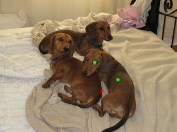
\includegraphics[width=\linewidth]{cap_comandos/figuras/interactive_example_a.png}\\
    (a)
\end{minipage}
\hfill
\begin{minipage}{0.32\linewidth}
    \centering
    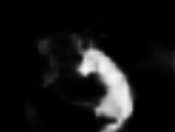
\includegraphics[width=\linewidth]{cap_comandos/figuras/interactive_example_b.png}\\
    (b)
\end{minipage}
\hfill
\begin{minipage}{0.32\linewidth}
    \centering
    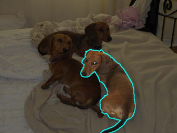
\includegraphics[width=\linewidth]{cap_comandos/figuras/interactive_example_c.png}\\
    (c)
\end{minipage}

\vspace{0.2cm}
{\small Fonte: \cite{xu2016deep_arxiv}}
\end{figure}


%O objetivo da segmentação de imagem interativa é obter uma acurácia próxima a da máscara do objeto usando o menos cliques possível do usuário. A maior parte dos métodos possui uma inferface onde o usuário pode realizar cliques positivos e cliques negativos diversas vezes, até que a máscara do objeto desejada seja obtida. \cite{sofiiuk2020fbrs_arxiv}

%Algumas abordagens utilizam o interactive learning para auxiliar no refinamento do modelo de segmentação, outros, utilizam para que o usuário escolha o objeto a ser segmentado, ou que para faça a correção pontual na segmentação da imagem gerada.



\section{Continual Learning}\label{sec_cl}

O aprendizado contínuo (\ac{CL}) constitui um subcampo da Inteligência Artificial dedicado ao desenvolvimento de modelos capazes de aprender de forma sequencial e incremental a partir de fluxos contínuos de dados, sem a necessidade de serem completamente retreinados a cada novo conjunto de informações. Essa habilidade de acumular conhecimento ao longo do tempo, característica intrínseca à inteligência biológica, permanece um desafio central para redes neurais artificiais \cite{delange2021continual}.

O principal obstáculo associado à \ac{CL} é o fenômeno conhecido como esquecimento catastrófico (catastrophic forgetting), no qual a atualização dos parâmetros do modelo para incorporar novos conhecimentos interfere negativamente no desempenho obtido em tarefas previamente aprendidas.

Diversos métodos têm sido propostos na literatura para mitigar esse problema. Entre eles, destacam-se três classes predominantes:

\begin{enumerate}

\item \textbf{Métodos baseados em regularização}: introduzem termos adicionais (penalidades) na função de perda com a finalidade de restringir alterações em parâmetros que foram identificados como essenciais para tarefas anteriores. Um exemplo notável dessa categoria é o \ac{EWC}, que estima a importância dos pesos e penaliza alterações proporcionais a essa relevância \cite{kirkpatrick2017overcoming}.

\item \textbf{Métodos baseados em replay}: consistem em preservar um subconjunto reduzido dos dados de tarefas passadas e reexibi-los ao modelo durante o treinamento de novas tarefas, evitando que antigos conhecimentos sejam sobrescritos. O método iCaRL, por exemplo, emprega conjuntos representativos de exemplares para reter desempenho histórico ao longo das iterações de aprendizagem \cite{rebuffi2017icarl}.

\item \textbf{Métodos baseados em Destilação de Conhecimento}: introduzidos inicialmente por \cite{hinton2015distilling}, tratam o processo de transferência de conhecimento de um modelo para outro de forma análoga à relação professor-aluno. A estratégia consiste em induzir o modelo aluno a imitar não apenas as decisões finais do modelo professor, mas também sua distribuição de probabilidades, preservando informações relevantes mesmo diante de novos dados.
\end{enumerate}

No contexto deste trabalho, opta-se prioritariamente pela terceira abordagem, fundamentada em destilação de conhecimento, uma vez que ela se mostra particularmente adequada ao cenário interativo e incremental considerado, permitindo preservar conhecimento previamente adquirido durante a incorporação progressiva de novos exemplos.

%A Aprendizagem Contínua (\ac{CL}) é uma subárea da inteligência artificial que visa desenvolver modelos capazes de aprender de forma sequencial e incremental a partir de um fluxo contínuo de dados, sem a necessidade de serem retreinados do zero. Esta capacidade de acumular conhecimento ao longo do tempo é uma característica fundamental da inteligência biológica, mas representa um desafio significativo para as redes neurais artificiais \cite{delange2021continual}.

%Um dos principais obstáculos a ser superado é o chamado esquecimento carastrófico (catastrophic forgetting), onde o ajuste dos pesos do modelo ao aprender uma nova tarefa, interfere com o conhecimento que o modelo adquiriu anteriormente, alterando a performance em tarefas antigas.

%Para mitigar esse problema, foram propostas diversas abordagens, dentre elas, três se destacam: 

%\begin{enumerate}
%\item Abordagens baseadas em regularização: essa abordagem adiciona uma penalidade na função de perda, o que evita a atualização dos pesos considerados importantes para as tarefas antigas. A estratégia mais proeminente aqui é a Abordagem de Consolidação Elástica de Pesos, na qual calcula a importância de cada peso e penaliza a sua modificação \cite{kirkpatrick2017overcoming}
%\item A segunda abordagem consiste em estratégias de replay: Armazena pequenos subconjunto de dados de tarefas antigas, apresentando ao modelo durante o treinamento de novas tarefas. Um dos exemplos dessa abordagem é o iCaRL, que utiliza exemplo de dados antigos para retreinar o modelo a cada nova etapa do conhecimento \cite{rebuffi2017icarl}.
%\item A terceira abordagem é a Destilação de Conhecimento: esse método foi criado por \cite{hinton2015distilling}, como um modelo de passagem de conhecimento analogo a um professor e um aluno. A ideia é que o aluno aprenda a imitar as saídas do professor, não apenas as respostas finais, mas a distribuição de probabilidade completa.
%\end{enumerate}

%No presente trabalho, é adotada a abordagem de Destilação de Conhecimento.


\section{Feature Learning from Image Markers}

As redes convolucionais descritas até aqui ajustam seus filtros por retropropagação, o que exige grandes conjuntos anotados e capacidade computacional proporcional. O \ac{FLIM}, proposto por \cite{souza2020flim}, parte de uma premissa diferente: os filtros não são descobertos por otimização, e sim estimados a partir de marcadores que o especialista desenha sobre poucas imagens representativas.

O procedimento é estimar os filtros camada a camada. Para cada marcador, o método recorta os patches centrados nos pixels marcados, agrupa esses patches e usa os centróides resultantes como filtros daquela camada. A saída da camada serve de entrada para o mesmo procedimento na camada seguinte, de modo que a estimação avança sem nenhum passo de retropropagação e sem inicialização aleatória de pesos. Com isso, o especialista deixa de fornecer apenas rótulos e passa a indicar quais regiões da imagem discriminam o objeto.

A consequência prática é a redução drástica do número de imagens anotadas. Enquanto uma rede treinada por retropropagação costuma exigir milhares de exemplos, redes \ac{FLIM} são construídas a partir de uma a poucas imagens por classe \cite{benato2020cnnmarkers}. O método foi aplicado a delineamento de objetos \cite{souza2020flim} e a classificação de imagens de sensoriamento remoto \cite{souza2020coconut}, com resultados comparáveis e às vezes superiores aos da mesma arquitetura treinada do zero.

\subsection{Decodificadores adaptativos}

Um encoder \ac{FLIM} produz mapas de ativação, não uma máscara de segmentação. É preciso então converter esses mapas em uma decisão por pixel. \cite{soares2026flim} propõem decodificadores adaptativos para essa conversão: em vez de aprender um decodificador fixo, os pesos são calculados para cada imagem de entrada por uma função heurística que estima se cada canal de ativação responde ao objeto ou ao fundo.

Essa escolha mantém a rede leve, porque o decodificador é uma convolução ponto a ponto com pesos em $\{-1, +1\}$, e preserva a propriedade central do \ac{FLIM}: nenhum parâmetro é ajustado por gradiente. O trabalho relata redes centenas de vezes menores que modelos considerados leves, treinadas com três a quatro imagens representativas. Trabalhos subsequentes na mesma linha exploram kernels separáveis dilatados para reduzir ainda mais o número de parâmetros \cite{joao2025flyweight}.

É esse arranjo, encoder \ac{FLIM} com decodificador adaptativo, que o presente trabalho reproduz e sobre o qual aplica as estratégias de aprendizado ativo, interativo e contínuo descritas nas seções anteriores.

\subsection{Por que a combinação com AL e CL não é imediata}

As três estratégias discutidas neste capítulo pressupõem, de formas diferentes, um modelo treinado por gradiente.

O \ac{AL} supõe que o modelo melhora de maneira previsível quando recebe rótulos adicionais, e por isso faz sentido escolher quais exemplos rotular. O \ac{CL} supõe que o esquecimento catastrófico decorre do deslocamento dos pesos durante o ajuste por gradiente, e as três classes de método descritas na Seção \ref{sec_cl} combatem exatamente esse deslocamento: regularização penaliza a mudança de pesos importantes, replay reapresenta dados antigos ao otimizador, e destilação faz o modelo aluno imitar as saídas do professor. Nenhuma dessas operações está definida para um modelo sem otimizador.

No \ac{FLIM} a relação entre anotação e parâmetros é de outra natureza. Os filtros são centróides de agrupamentos sobre os patches marcados, e o banco de filtros é compartilhado por todas as imagens, inclusive as não anotadas. Acrescentar marcadores altera o conjunto de patches candidatos, o que altera o agrupamento e, por consequência, os filtros já estimados. A anotação adicional, portanto, não refina o modelo de forma incremental: ela reestima o extrator de atributos.

Essa diferença é o ponto de partida da metodologia apresentada no Capítulo \ref{cap_3}, e a sua caracterização quantitativa é o objeto dos experimentos relatados no Capítulo \ref{cap_4}.


\section{Trabalhos Relacionados}

Conforme discutido anteriormente (Seção \ref{cap_1}), a literatura apresenta uma ampla variedade de estratégias e métodos voltados à potencialização de modelos de Inteligência Artificial, buscando equilibrar custo computacional, tempo de treinamento e desempenho preditivo. Em linhas gerais, os estudos diferenciam-se pelas abordagens adotadas para mitigar limitações recorrentes, tais como o tempo elevado de processamento, escassez de dados anotados, necessidade de maior acurácia e a integração de mecanismos avançados de aprendizagem, incluindo \ac{AL}, \ac{CL}, \ac{IL}, arquiteturas híbridas, novos algoritmos, introdução de adaptadores, otimizações em transformers, entre outros.
%Nesse contexto, é apresentada a Tabela \ref{tab:trabalhos_relacionados} com os principais trabalhos relacionados, organizada de modo a caracterizar cada proposta quanto à sua abordagem central, bem como destacar suas principais vantagens e limitações.

%Conforme visto anteriormente (Seção 1), há diversas estratégias e métodos para que um modelo de Inteligência Artificial seja potencializado, equilibrando métricas de custo computacional e tempo gasto. Em geral, os trabalhos destacam-se pelas diferentes abordagens afim de melhorar as lacunas existentes, como a demora de execução de um modelo, falta de dados, melhorias de acurácia e aplicações de métodos diversos, como \ac{AL}, \ac{CL}, \ac{IL}, mistura de abordagens, novos algoritmos, adaptadores, melhorias nos transformers, entre outros. A seguir, apresenta-se uma tabela dos principais trabalhos relacionados, caracterizando-os conforme sua abordagem, vantagens e desvantagens de cada um. 

% \begin{table}[h!]
% \centering
% \caption{Trabalhos relacionados à segmentação de imagens.}
% \label{tab:trabalhos_relacionados}
% \tiny
% \begin{adjustbox}{angle=90}
% \begin{tabular}{|c|l|l|l|l|c|c|}
% \hline
% \textbf{Nº} & \textbf{Autores} & \textbf{Técnica Principal} & \textbf{Algoritmo/Modelo} & \textbf{Dataset(s)} & \textbf{AL} & \textbf{VLM} \\\hline
% 1 & \cite{stutz2018superpixels} & Survey (Superpixels) & Taxonomia de superpixels & BSDS500, NYUV2, SUNRGBD & - & - \\\hline
% 2 & \cite{hesamian2020medical} & Survey (Medicina) & Revisão DL médica & - & - & - \\\hline
% 3 & \cite{jha2020kvasirseg} & Arquitetura CNN & U-Net, variantes & Kvasir-SEG & - & - \\\hline
% 4 & \cite{emara2019liteseg} & Arquitetura CNN (Leve) & LiteSeg (ASPP, depthwise) & Cityscapes & - & - \\\hline
% 5 & \cite{zhang2023attention} & Arquitetura CNN (Atenção) & SE-ASPP & Cityscapes, CamVid & - & - \\\hline
% 6 & \cite{wang2021boundary} & Estratégia (Função de Perda) & Boundary Loss & Cityscapes & - & - \\\hline
% 7 & \cite{liao2023dual} & Estratégia (Label Noise) & Dual-task Crowd Labels & Cityscapes, CamVid & - & - \\\hline
% 8 & \cite{gansbeke2021unsupervised} & Estratégia (Aprend. Contrastiva) & Object Mask Contrast & Cityscapes, \ac{PascalPascalVOC2012}& - & - \\\hline
% 9 & \cite{yang2018curriculum} & Estratégia (Adaptação de Domínio) & Curriculum Adaptation & Cityscapes & - & - \\\hline
% 10 & \cite{hoffman2016unsupervised} & Estratégia (Adaptação de Domínio) & Adversarial Training & Cityscapes & - & - \\\hline
% 11 & \cite{zhang2019spda} & Estratégia (Aumento c/ Superpixel) & \ac{SLIC} + U-Net & BraTS, Nuclei, LiTS, CVC-ClinicDB & - & - \\\hline
% 12 & \cite{franchi2021robust} & Estratégia (Aumento c/ Superpixel) & DeepLabv3+ & Cityscapes & - & - \\\hline
% 13 & \cite{zhang2020dualwindow} & Estratégia (Aumento c/ Superpixel) & Dual-Window Aug. & PaviaU, Salinas & - & - \\\hline
% 14 & \cite{delarosa2022improving} & Estratégia (Aumento Sintético) & DeepLab V2, Xception & Cityscapes & - & - \\\hline
% 15 & \cite{baranchuk2021label} & Estratégia (Semi-supervisão) & DDPMs + seg. & Cityscapes & - & - \\\hline
% 16 & \cite{wang2020solo} & Técnica (Seg. de Instância) & SOLO & - & - & - \\\hline
% 17 & \cite{han2020dvsnet} & Técnica (Seg. de Vídeo) & DVSNet (Path decision) & Cityscapes & - & - \\\hline
% 18 & \cite{wu2023medical} & VLM (Adaptação c/ Adapter) & Medical SAM Adapter & PIPO-FAN, REFUGE2, ISIC, etc. & - & \checkmark \\\hline
% 19 & \cite{huang2024adapting} & VLM (Adaptação c/ Adapter) & Residual adapters & BrainMRI, LiverCT, RESC & - & \checkmark \\\hline
% 20 & \cite{gowda2024ccsam} & VLM (Fusão CNN+VLM) & CC-SAM (CNN + SAM) & TN3K, DDTI, TG3K, BUSI, etc. & - & \checkmark \\\hline
% 21 & \cite{koleilat2024medclipsamv2} & VLM (Fusão Multimodal) & MedCLIP-SAMv2 & ROCO, MedPix, BUSI, etc. & - & \checkmark \\\hline
% 22 & \cite{liu2024grounded} & VLM (Fusão Open-World) & SAM + Grounding DINO & COCO, LVIS, ADE20K, VG & - & \checkmark \\\hline
% 23 & \cite{xie2022ripu} & AL (Estratégia: Incerteza) & RIPU & Cityscapes & \checkmark & - \\\hline
% 24 & \cite{zheng2024alintro} & AL (Estratégia: Incerteza) & AL-Intro (SOD) & NJU2K, NLPR, SIP, STERE & \checkmark & - \\\hline
% 25 & \cite{konyushkova2017learning} & AL (Estratégia: Meta-Learning) & Meta-AL strategy & USPS, MNIST, BioID & \checkmark & - \\\hline
% 26 & \cite{kim2023adaptive} & AL (Estratégia: Baseada em Região) & Adaptive Superpixel (MCLU) & Cityscapes, \ac{PascalPascalVOC2012}& \checkmark & - \\\hline
% 27 & \cite{mackowiak2018cereals} & AL (Estratégia: Baseada em Região) & CEREALS (superpixels) & Cityscapes & \checkmark & - \\\hline
% 28 & \cite{rangnekar2022region} & AL (Estratégia: Baseada em Região) & Teacher-Student & Cityscapes, CamVid & \checkmark & - \\\hline
% 29 & \cite{franco2023halo} & AL (Estratégia: Otimização HW) & HALO & Cityscapes (GTAV sintético) & \checkmark & - \\\hline
% 30 & \cite{casanova2020reinforced} & AL (Híbrido: AL + RL) & DQN (seleção de regiões) & Cityscapes, CamVid & \checkmark & - \\\hline
% 31 & \cite{rangnekar2022mean} & AL (Híbrido: AL + Semi-sup.) & Mean Teacher + Contrastive & Cityscapes, CamVid & \checkmark & - \\\hline
% 32 & \cite{karamcheti2021dial} & AL (Híbrido: AL + IL) & DIAL (Bayesiana) & ISPRS Vaihingen, \ac{PascalVOC2012}& \checkmark & - \\\hline
% 33 & \cite{triebel2014active} & AL (Híbrido: AL + IL Online) & Sparse GPs & GrabCut & \checkmark & - \\\hline
% 34 & \cite{vu2023active} & AL (Híbrido: AL + CL) & CL + Acquisition Function & ASC + 20News & \checkmark & - \\\hline
% 35 & \cite{zheng2021continual} & CL (Híbrido: CL + IL) & Continual + Uncertainty & ISIC, CHAOS, \ac{PascalVOC2012}& \checkmark & - \\\hline
% \end{tabular}
% \end{adjustbox}
% \end{table}

\begin{table}[h!]
\centering
\caption{Trabalhos relacionados à segmentação de imagens}% com colunas adicionais para IL e CL.}
\label{tab:trabalhos_relacionados}
\tiny
\begin{adjustbox}{angle=90, max height=\textheight}
\begin{tabular}{|c|l|l|l|l|c|c|c|c|}
\hline
\textbf{Nº} & \textbf{Autores} & \textbf{Técnica Principal} & \textbf{Algoritmo/Modelo} & \textbf{Dataset(s)} & \textbf{AL} & \textbf{VLM} & \textbf{IL} & \textbf{CL} \\\hline

1 & \cite{stutz2018superpixels} & Survey (Superpixels) & Taxonomia de superpixels & BSDS500, NYUV2, SUNRGBD & - & - & - & - \\\hline
2 & \cite{hesamian2020medical} & Survey (Medicina) & Revisão DL médica & - & - & - & - & - \\\hline
3 & \cite{jha2020kvasirseg} & Arquitetura CNN & U-Net, variantes & Kvasir-SEG & - & - & - & - \\\hline
4 & \cite{emara2019liteseg} & Arquitetura CNN (Leve) & LiteSeg (ASPP, depthwise) & Cityscapes & - & - & - & - \\\hline
5 & \cite{zhang2023attention} & Arquitetura CNN (Atenção) & SE-ASPP & Cityscapes, CamVid & - & - & - & - \\\hline
6 & \cite{wang2021boundary} & Estratégia (Função de Perda) & Boundary Loss & Cityscapes & - & - & - & - \\\hline
7 & \cite{liao2023dual} & Estratégia (Label Noise) & Dual-task Crowd Labels & Cityscapes, CamVid & - & - & - & - \\\hline
8 & \cite{gansbeke2021unsupervised} & Estratégia (Aprend. Contrastiva) & Object Mask Contrast & Cityscapes, \ac{PascalVOC2012}& - & - & - & - \\\hline
9 & \cite{yang2018curriculum} & Estratégia (Adaptação de Domínio) & Curriculum Adaptation & Cityscapes & - & - & - & - \\\hline
10 & \cite{hoffman2016unsupervised} & Estratégia (Adaptação de Domínio) & Adversarial Training & Cityscapes & - & - & - & - \\\hline
11 & \cite{zhang2019spda} & Estratégia (Aumento c/ Superpixel) & \ac{SLIC} + U-Net & BraTS, Nuclei, LiTS, CVC-ClinicDB & - & - & - & - \\\hline
12 & \cite{franchi2021robust} & Estratégia (Aumento c/ Superpixel) & DeepLabv3+ & Cityscapes & - & - & - & - \\\hline
13 & \cite{zhang2020dualwindow} & Estratégia (Aumento c/ Superpixel) & Dual-Window Aug. & PaviaU, Salinas & - & - & - & - \\\hline
14 & \cite{delarosa2022improving} & Estratégia (Aumento Sintético) & DeepLab V2, Xception & Cityscapes & - & - & - & - \\\hline
15 & \cite{baranchuk2021label} & Estratégia (Semi-supervisão) & DDPMs + seg. & Cityscapes & - & - & - & - \\\hline
16 & \cite{wang2020solo} & Técnica (Seg. de Instância) & SOLO & - & - & - & - & - \\\hline
17 & \cite{han2020dvsnet} & Técnica (Seg. de Vídeo) & DVSNet (Path decision) & Cityscapes & - & - & - & - \\\hline
18 & \cite{wu2023medical} & VLM (Adaptação c/ Adapter) & Medical SAM Adapter & PIPO-FAN, REFUGE2, ISIC, etc. & - & \checkmark & - & - \\\hline
19 & \cite{huang2024adapting} & VLM (Adaptação c/ Adapter) & Residual adapters & BrainMRI, LiverCT, RESC & - & \checkmark & - & - \\\hline
20 & \cite{gowda2024ccsam} & VLM (Fusão CNN+VLM) & CC-SAM & TN3K, DDTI, TG3K, BUSI, etc. & - & \checkmark & - & - \\\hline
21 & \cite{koleilat2024medclipsamv2} & VLM (Fusão Multimodal) & MedCLIP-SAMv2 & ROCO, MedPix, BUSI, etc. & - & \checkmark & - & - \\\hline
22 & \cite{liu2024grounded} & VLM (Fusão Open-World) & SAM + Grounding DINO & COCO, LVIS, ADE20K, VG & - & \checkmark & - & - \\\hline
23 & \cite{xie2022ripu} & AL (Estratégia: Incerteza) & RIPU & Cityscapes & \checkmark & - & - & - \\\hline
24 & \cite{zheng2024alintro} & AL (Estratégia: Incerteza) & AL-Intro (SOD) & NJU2K, NLPR, SIP, STERE & \checkmark & - & - & - \\\hline
25 & \cite{konyushkova2017learning} & AL (Meta-Learning) & Meta-AL strategy & USPS, MNIST, BioID & \checkmark & - & - & - \\\hline
26 & \cite{kim2023adaptive} & AL (Região) & Adaptive Superpixel (MCLU) & Cityscapes, \ac{PascalVOC2012}& \checkmark & - & - & - \\\hline
27 & \cite{mackowiak2018cereals} & AL (Região) & CEREALS (superpixels) & Cityscapes & \checkmark & - & - & - \\\hline
28 & \cite{rangnekar2022region} & AL (Região) & Teacher-Student & Cityscapes, CamVid & \checkmark & - & - & - \\\hline
29 & \cite{franco2023halo} & AL (Otimização HW) & HALO & Cityscapes (GTAV sintético) & \checkmark & - & - & - \\\hline
30 & \cite{casanova2020reinforced} & AL + RL & DQN (seleção de regiões) & Cityscapes, CamVid & \checkmark & - & - & - \\\hline
31 & \cite{rangnekar2022mean} & AL + Semi-Sup. & Mean Teacher + Contrastive & Cityscapes, CamVid & \checkmark & - & - & - \\\hline
32 & \cite{karamcheti2021dial} & AL + IL & DIAL (Bayesiana) & ISPRS Vaihingen, \ac{PascalVOC2012}& \checkmark & - & \checkmark & - \\\hline
33 & \cite{triebel2014active} & AL + IL Online & Sparse GPs & GrabCut & \checkmark & - & \checkmark & - \\\hline
34 & \cite{vu2023active} & AL + CL & CL + Acquisition Function & ASC + 20News & \checkmark & - & - & \checkmark \\\hline
35 & \cite{zheng2021continual} & CL + IL & Continual + Uncertainty & ISIC, CHAOS, \ac{PascalVOC2012}& - & - & \checkmark & \checkmark \\\hline
\end{tabular}
\end{adjustbox}
\end{table}


\begin{table}[h!]
\centering
\caption{Síntese dos principais datasets públicos reportados na literatura e utilizados como referência para treinamento e avaliação em segmentação semântica.}
\label{tab:datasets}
\tiny
\begin{adjustbox}{angle=90}
\begin{tabular}{|c|l|l|l|l|c|c|c|}
\hline
\textbf{Nº} & \textbf{Nome} & \textbf{Tamanho} & \textbf{Número de imagens} & \textbf{Resolução} & \textbf{Número de classes} & \textbf{Tipo de imagens} & \textbf{Ano} \\ \hline

1 & \ac{PascalVOC2012} & 4 GB & 11.530 (treino/val) & 500x375 & 20 & Segmentação de Objetos & 2012 \\ \hline
2 & Cityscapes & 25 GB & 5.000  & 2048x1024 & 30 & Cenas Urbanas & 2016 \\ \hline
3 & CamVid & 570 MB & 701 frames & 960x720 & 32 & Cenas Urbanas (Vídeo) & 2008 \\ \hline
4 & COCO & 50 GB & 330.000 & Variável & 80 & Segmentação de Objetos & 2014 \\ \hline
5 & LVIS & 25 GB & 164.000 & Variável & 1.203 & Segmentação de Instâncias & 2019 \\ \hline
6 & ADE20K & 3 GB & 27.000 & Variável & 150 & Análise de Cenas & 2016 \\ \hline
7 & GTA V (Sintético) & 180 GB & 25.000 & 1914x1052 & 19 & Cenas Urbanas (Sintético) & 2016 \\ \hline
8 & NYU Depth V2 & 5.5 GB & 1.449 & 640x480 & 40 & Cenas Internas (RGB-D) & 2012 \\ \hline
9 & SUN RGB-D & 60 GB & 10.335 & Variável & 37 & Cenas Internas (RGB-D) & 2015 \\ \hline
10 & NLPR & ~1 GB & 1.000 pares & 640x480 & 1 & Detecção de Obj. Salientes & 2014 \\ \hline
11 & NJU2K & 1.5 GB & 1.985 pares & Variável & 1 & Detecção de Objetos & 2014 \\ \hline
12 & STERE & 100 MB & 1.000 pares & 1024x768 & 1 & Detecção de Objetos (Estéreo) & 2015 \\ \hline
13 & Kvasir-SEG & 2 GB & 1.000 & 576x720 & 1 & Médica (Pólipo Colorretal) & 2020 \\ \hline
14 & BraTS & 200 GB & ~3.000 (3D) & 240x240x155 & 3 & Médica 3D (Tumor Cerebral) & 2012 \\ \hline
15 & LiTS / LiverCT & 80 GB & 131 scans CT & 512x512xZ & 2 & Médica 3D (Fígado) & 2017 \\ \hline
16 & CVC-ClinicDB & 50 MB & 612 & 384x288 & 1 & Médica (Endoscopia) & 2015 \\ \hline
17 & REFUGE2 & 3.8 GB & 1.200 & UHD (várias) & 2 & Médica (Oftalmologia) & 2020 \\ \hline
18 & ISIC & Variável & > 203.000 & Variável & 2-7 & Médica (Dermatologia) & 2016 \\ \hline
19 & BrainMRI & 350 MB & 3.929 & 256x256 & 1 & Médica (Tumor Cerebral) & 2020 \\ \hline
20 & RESC & 500 MB & 110 scans & Variável & 3 & Médica (Edema Retinal) & 2018 \\ \hline
21 & TN3K & 200 MB & 3.500 & 400x400 & 1 & Médica (Nódulo Tireoide) & 2022 \\ \hline
22 & DDTI & 1.5 GB & 5.000 & Variável & 1 & Médica (Raio-X Panorâmico) & 2022 \\ \hline
23 & TG3K & 250 MB & 3.100 & 400x400 & 1 & Médica (Glândula Tireoide) & 2022 \\ \hline
24 & BUSI & 250 MB & 780 & ~500x500 & 3 & Médica (Ultrassom de Mama) & 2019 \\ \hline
25 & CHAOS & 20 GB & 80 scans & 512x512xZ & 4 & Médica 3D (Abdômen) & 2019 \\ \hline
26 & ISPRS Vaihingen & 2 GB & 33 & ~2500x2000 & 6 & Imagens Aéreas & 2012 \\ \hline
27 & PaviaU & 100 MB & 1 (hiperespectral) & 610x340x103 & 9 & Imagens Hiperespectrais & - \\ \hline
28 & 300W-LP & 4 GB & 122.450 & Variável & 68 (pontos) & Detecção de Pontos Faciais & 2016 \\ \hline
29 & BioID & 150 MB & 1.521 & 384x288 & 1 & Detecção de Face & 1999 \\ \hline
30 & USPS & 10 MB & 9.298 & 16x16 & 10 & Classificação (Manuscritos) & 1990 \\ \hline
31 & MNIST & 15 MB & 70.000 & 28x28 & 10 & Classificação (Manuscritos) & 1998 \\ \hline
32 & ROCO & 8 GB & 81.000 & Variável & N/A & Legenda de Imagens Médicas & 2018 \\ \hline
33 & MedPix & Variável & 59.000 & Variável & N/A & Banco de Imagens Médicas & 1999 \\ \hline
34 & Visual Genome (VG) & 12 GB & 108.000 & Variável & N/A & Legenda de Imagens & 2016 \\ \hline
35 & Nuclei Dataset & 100 MB & 30.000 patches & ~50x50 & 1 & Biomédica (Núcleos Celulares) & 2018 \\ \hline
36 & BSDS500 & 100 MB & 500 & Variável & N/A & Detecção de Contorno & ~2011 \\ \hline
37 & GrabCut & 5 MB & 50 & Variável & 1 & Segmentação Interativa & 2004 \\ \hline
38 & LIDS/UNICAMP & \textasciitilde 500 MB & 6.943 & Variável & 21 & Médica (Parasitas Intestinais, Microscopia) & 2023 \\ \hline


\end{tabular}
\end{adjustbox}
\end{table}


%  -----------------------
% N° dos Artigos seguidos como base (Implementações a partir dos códigos fornecidos): 
% 03 (Superpixel)
% 23 (Casanova)
% 33 (Zheng)
% 34 (Triebel)
% 35 (Vu)
%  -----------------------

% \begin{table}[h!]
% \caption{Tabela de Trabalhos Relacionados\label{tab:trabalhos_relacionados}}\\
% \centering
% \tiny
% \begin{adjustbox}{angle=90}
% \begin{tabular}{ccccccc}
% \hline
% \textbf{Autores} & \textbf{Aumento} & \textbf{Conjunto} & \textbf{Extração} & \textbf{Classificação} & \textbf{AL} & \textbf{viés}\\\hline

% \end{tabular}
% \end{adjustbox}
% \end{table}


% \newcolumntype{L}[1]{>{\raggedright\arraybackslash\hspace{0pt}}p{#1\linewidth}}
% \newcolumntype{C}[1]{>{\centering\arraybackslash\hspace{0pt}}p{#1\linewidth}}


% \begin{longtable}{C{0.04} L{0.20} L{0.66}}

% \caption{Tabela de Trabalhos Relacionados\label{tab:trabalhos_relacionados}}\\
% \toprule
% \textbf{Nº} & \textbf{Referência} & \textbf{Detalhes Técnicos} \\
% \midrule
% \endfirsthead

% \multicolumn{3}{c}{{\bfseries \tablename\ \thetable{} -- continuação}} \\
% \toprule
% \textbf{Nº} & \textbf{Referência} & \textbf{Detalhes Técnicos} \\
% \midrule
% \endhead

% \bottomrule
% \multicolumn{3}{r@{}}{Continua na próxima página...} \\
% \endfoot

% \endlastfoot

% \multicolumn{3}{l}{\textbf{\large Categoria: Trabalhos sem Aprendizagem Ativa}} \\
% \midrule

% 1 & \cite{jha2020kvasirseg}
% & \textbf{Título:} Kvasir-SEG: A Segmented Polyp Dataset \newline
%   \textbf{Técnica Principal:} CNN \quad \textbf{VLM:} Não \newline
%   \textbf{Algoritmo:} U-Net e variantes para segmentação de pólipos. \newline
%   \textbf{Datasets:} Kvasir-SEG.
% \\ \midrule

% 2 & \cite{zhang2019spda}
% & \textbf{Título:} SPDA: Superpixel-based Data Augmentation \newline
%   \textbf{Técnica Principal:} Aumento de Dados (Superpixel) \quad \textbf{VLM:} Não \newline
%   \textbf{Algoritmo:} Geração de novas amostras de treino com base em superpixels (\ac{SLIC} + U-Net). \newline
%   \textbf{Datasets:} BraTS, Nuclei, LiTS, CVC-ClinicDB.
% \\ \midrule

% 3 & \cite{franchi2021robust}
% & \textbf{Título:} Robust Semantic Segmentation with Superpixel-Mix \newline
%   \textbf{Técnica Principal:} Aumento de Dados (Superpixel) \quad \textbf{VLM:} Não \newline
%   \textbf{Algoritmo:} DeepLabv3+ com a técnica Superpixel-Mix. \newline
%   \textbf{Datasets:} Cityscapes.
% \\ \midrule

% 4 & \cite{zhang2020dualwindow}
% & \textbf{Título:} Dual-Window Superpixel Data Augmentation \newline
%   \textbf{Técnica Principal:} Aumento de Dados (Superpixel) \quad \textbf{VLM:} Não \newline
%   \textbf{Algoritmo:} Aumento de dados para imagens hiperespectrais. \newline
%   \textbf{Datasets:} PaviaU, Salinas.
% \\ \midrule

% 5 & \cite{stutz2018superpixels}
% & \textbf{Título:} Superpixels: An Evaluation of the State-of-the-Art \newline
%   \textbf{Técnica Principal:} Survey \quad \textbf{VLM:} Não \newline
%   \textbf{Contribuição:} Avaliação e taxonomia de algoritmos de superpixel. \newline
%   \textbf{Datasets:} BSDS500, NYUV2, SUNRGBD.
% \\ \midrule

% 6 & \cite{wang2021boundary}
% & \textbf{Título:} Boundary-Loss for Semantic Segmentation \newline
%   \textbf{Técnica Principal:} Função de Perda \quad \textbf{VLM:} Não \newline
%   \textbf{Algoritmo:} Proposta de uma função de perda focada em bordas. \newline
%   \textbf{Datasets:} Cityscapes.
% \\ \midrule

% 7 & \cite{liao2023dual}
% & \textbf{Título:} Dual-task Annotation-free Learning from Crowds \newline
%   \textbf{Técnica Principal:} Aprendizagem com Ruído \quad \textbf{VLM:} Não \newline
%   \textbf{Algoritmo:} Aprendizagem a partir de anotações de crowdsourcing. \newline
%   \textbf{Datasets:} Cityscapes, CamVid.
% \\ \midrule

% 8 & \cite{zhang2023attention}
% & \textbf{Título:} Attention-calibrated SE-ASPP for Seg. \newline
%   \textbf{Técnica Principal:} Arquitetura de Rede (Atenção) \quad \textbf{VLM:} Não \newline
%   \textbf{Algoritmo:} Proposta de arquitetura com Attention e SE-ASPP. \newline
%   \textbf{Datasets:} Cityscapes, CamVid.
% \\ \midrule

% 9 & \cite{gansbeke2021unsupervised}
% & \textbf{Título:} Unsupervised Seg. by Contrasting Object Mask Proposals \newline
%   \textbf{Técnica Principal:} Aprendizagem Contrastiva \quad \textbf{VLM:} Não \newline
%   \textbf{Algoritmo:} Segmentação não-supervisionada via contraste de máscaras. \newline
%   \textbf{Datasets:} Cityscapes, VOC.
% \\ \midrule

% 10 & \cite{yang2018curriculum}
% & \textbf{Título:} Curriculum Domain Adaptation for Semantic Seg. \newline
%   \textbf{Técnica Principal:} Adaptação de Domínio \quad \textbf{VLM:} Não \newline
%   \textbf{Algoritmo:} Adaptação com estratégia de currículo (sintético para real). \newline
%   \textbf{Datasets:} Cityscapes.
% \\ \midrule

% 11 & \cite{hoffman2016unsupervised}
% & \textbf{Título:} Unsupervised Domain Adaptation for Semantic Seg. \newline
%   \textbf{Técnica Principal:} Adaptação de Domínio \quad \textbf{VLM:} Não \newline
%   \textbf{Algoritmo:} Adaptação não-supervisionada com adversarial training. \newline
%   \textbf{Datasets:} Cityscapes.
% \\ \midrule

% 12 & \cite{emara2019liteseg}
% & \textbf{Título:} LiteSeg: A Novel Lightweight ConvNet \newline
%   \textbf{Técnica Principal:} Arquitetura de Rede (Leve) \quad \textbf{VLM:} Não \newline
%   \textbf{Algoritmo:} CNN leve com ASPP e depthwise convolutions. \newline
%   \textbf{Datasets:} Cityscapes.
% \\ \midrule

% 13 & \cite{wang2020solo}
% & \textbf{Título:} SOLO: Segmenting objects by location \newline
%   \textbf{Técnica Principal:} Segmentação por Instância \quad \textbf{VLM:} Não \newline
%   \textbf{Algoritmo:} Proposta de método para segmentação de instância. \newline
%   \textbf{Datasets:} -
% \\ \midrule

% 14 & \cite{han2020dvsnet}
% & \textbf{Título:} DVSNet: Dynamic Video Segmentation Network \newline
%   \textbf{Técnica Principal:} Segmentação de Vídeo \quad \textbf{VLM:} Não \newline
%   \textbf{Algoritmo:} Path decision network para eficiência em vídeo. \newline
%   \textbf{Datasets:} Cityscapes.
% \\ \midrule

% 15 & \cite{baranchuk2021label}
% & \textbf{Título:} Label-efficient semantic segmentation with diffusion models \newline
%   \textbf{Técnica Principal:} Modelos de Difusão (DDPMs) \quad \textbf{VLM:} Não \newline
%   \textbf{Algoritmo:} Uso de DDPMs para segmentação semi-supervisionada. \newline
%   \textbf{Datasets:} Cityscapes.
% \\ \midrule

% 16 & \cite{delarosa2022improving}
% & \textbf{Título:} Improving semantic segmentation... by using synthetic images \newline
%   \textbf{Técnica Principal:} Aumento de Dados (Sintético) \quad \textbf{VLM:} Não \newline
%   \textbf{Algoritmo:} Uso de imagens sintéticas para treinar DeepLab V2/Xception. \newline
%   \textbf{Datasets:} Cityscapes.
% \\ \midrule

% 17 & \cite{hesamian2020medical}
% & \textbf{Título:} Medical Image Segmentation Using Deep Learning: A Survey \newline
%   \textbf{Técnica Principal:} Survey \quad \textbf{VLM:} Não \newline
%   \textbf{Contribuição:} Revisão de métodos de Deep Learning para segmentação médica. \newline
%   \textbf{Datasets:} -
% \\ \midrule

% 18 & \cite{wu2023medical}
% & \textbf{Título:} Medical SAM Adapter \newline
%   \textbf{Técnica Principal:} Adaptação de Modelo \quad \textbf{VLM:} SAM \newline
%   \textbf{Algoritmo:} Adaptação do SAM sem fine-tuning através de adaptadores. \newline
%   \textbf{Datasets:} PIPO-FAN, REFUGE2, TNMIX, ISIC, TNSCUI, DDTI.
% \\ \midrule

% 19 & \cite{huang2024adapting}
% & \textbf{Título:} Adapting V-L Models for Anomaly Detection \newline
%   \textbf{Técnica Principal:} Adaptação de Modelo \quad \textbf{VLM:} CLIP \newline
%   \textbf{Algoritmo:} Adaptação do CLIP com adaptadores residuais. \newline
%   \textbf{Datasets:} BrainMRI, LiverCT, RESC.
% \\ \midrule

% 20 & \cite{gowda2024ccsam}
% & \textbf{Título:} CC-SAM \newline
%   \textbf{Técnica Principal:} Fusão de Modelos \quad \textbf{VLM:} SAM \newline
%   \textbf{Algoritmo:} SAM com CNN, prompts contextuais e atenção cruzada. \newline
%   \textbf{Datasets:} TN3K, DDTI, TG3K, BUSI, UDIAT, CAMUS, HMC-QU.
% \\ \midrule

% 21 & \cite{koleilat2024medclipsamv2}
% & \textbf{Título:} MedCLIP-SAMv2 \newline
%   \textbf{Técnica Principal:} Fusão de Modelos (Text-Driven) \quad \textbf{VLM:} CLIP, SAM \newline
%   \textbf{Algoritmo:} Integração de CLIP e SAM com prompts de texto. \newline
%   \textbf{Datasets:} ROCO, MedPix, BUSI, UDIAT, COVID-QU-Ex, BrainTumors, Lung CT.
% \\ \midrule

% 22 & \cite{liu2024grounded}
% & \textbf{Título:} Grounded SAM \newline
%   \textbf{Técnica Principal:} Fusão de Modelos (Open-World) \quad \textbf{VLM:} SAM, Grounding DINO \newline
%   \textbf{Algoritmo:} Integração de SAM com o detector de objetos Grounding DINO. \newline
%   \textbf{Datasets:} COCO, LVIS, Visual Genome, ADE20K.
% \\ \midrule

% \multicolumn{3}{l}{\textbf{\large Categoria: Trabalhos com Aprendizagem Ativa e Interativa}} \\
% \midrule

% 23 & \cite{casanova2020reinforced}
% & \textbf{Título:} Reinforced Active Learning for Image Segmentation \newline
%   \textbf{Técnica Principal:} Aprendizado por Reforço \quad \textbf{VLM:} Não \newline
%   \textbf{Abordagem de AL:} Seleção de regiões via RL com Deep Q-Network (DQN). \newline
%   \textbf{Datasets:} Cityscapes, CamVid.
% \\ \midrule

% 24 & \cite{xie2022ripu}
% & \textbf{Título:} RIPU: Region Impurity and Prediction Uncertainty \newline
%   \textbf{Técnica Principal:} Estratégia de Incerteza \quad \textbf{VLM:} Não \newline
%   \textbf{Abordagem de AL:} Baseada em Incerteza de Região e de Predição. \newline
%   \textbf{Datasets:} Cityscapes.
% \\ \midrule

% 25 & \cite{kim2023adaptive}
% & \textbf{Título:} Adaptive Superpixel for Active Learning \newline
%   \textbf{Técnica Principal:} Superpixel \quad \textbf{VLM:} Não \newline
%   \textbf{Abordagem de AL:} Com Superpixels adaptativos e critério de incerteza (MCLU). \newline
%   \textbf{Datasets:} Cityscapes, \ac{PascalVOC2012}.
% \\ \midrule

% 26 & \cite{konyushkova2017learning}
% & \textbf{Título:} Learning Active Learning from Data \newline
%   \textbf{Técnica Principal:} Data-Driven \quad \textbf{VLM:} Não \newline
%   \textbf{Abordagem de AL:} Aprende a própria estratégia de seleção a partir dos dados. \newline
%   \textbf{Datasets:} USPS, MNIST, BioID.
% \\ \midrule

% 27 & \cite{karamcheti2021dial}
% & \textbf{Título:} DIAL: Deep Interactive And Active Learning \newline
%   \textbf{Técnica Principal:} Bayesiana \quad \textbf{VLM:} Não \newline
%   \textbf{Abordagem:} Combina Aprendizagem Ativa (Incerteza Bayesiana) e Interativa. \newline
%   \textbf{Datasets:} ISPRS Vaihingen, \ac{PascalVOC2012}.
% \\ \midrule

% 28 & \cite{mackowiak2018cereals}
% & \textbf{Título:} CEREALS: Cost-Effective REgion-based AL \newline
%   \textbf{Técnica Principal:} Baseada em Região \quad \textbf{VLM:} Não \newline
%   \textbf{Abordagem de AL:} Seleção de superpixels baseada em custo-benefício. \newline
%   \textbf{Datasets:} Cityscapes.
% \\ \midrule

% 29 & \cite{rangnekar2022mean}
% & \textbf{Título:} Active Learning with Mean Teacher + Contrastive \newline
%   \textbf{Técnica Principal:} Semi-Supervisionada \quad \textbf{VLM:} Não \newline
%   \textbf{Abordagem de AL:} Com Mean Teacher e aprendizagem contrastiva. \newline
%   \textbf{Datasets:} Cityscapes, CamVid.
% \\ \midrule

% 30 & \cite{rangnekar2022region}
% & \textbf{Título:} Region-Based Active Learning \newline
%   \textbf{Técnica Principal:} Baseada em Região \quad \textbf{VLM:} Não \newline
%   \textbf{Abordagem de AL:} Com Teacher-Student e query de região. \newline
%   \textbf{Datasets:} Cityscapes, CamVid.
% \\ \midrule

% 31 & \cite{franco2023halo}
% & \textbf{Título:} HALO: Hardware-Aware Learning-to-Optimize for AL \newline
%   \textbf{Técnica Principal:} Otimização (Hardware-Aware) \quad \textbf{VLM:} Não \newline
%   \textbf{Abordagem de AL:} Otimiza a estratégia de seleção com base em restrições de hardware. \newline
%   \textbf{Datasets:} Cityscapes (sintetizado com GTAV).
% \\ \midrule
% 32 & \cite{zheng2024alintro}
% & \textbf{Título:} AL-Intro: Active Learning for Introduction-based SOD \newline
%   \textbf{Técnica Principal:} Estratégia de Incerteza \quad \textbf{VLM:} Não \newline
%   \textbf{Abordagem de AL:} Baseada na incerteza da introdução do objeto para Detecção de Objeto Saliente (SOD). \newline
%   \textbf{Datasets:} NJU2K, NLPR, STERE, SIP.
% \\ \midrule

% 33 & \cite{zheng2021continual}
% & \textbf{Título:} A Continual Learning Framework for Uncertainty-Aware Interactive Image Segmentation \newline
%   \textbf{Técnica Principal:} Aprendizagem Contínua e Interativa \quad \textbf{VLM:} Não \newline
%   \textbf{Abordagem:} Framework que combina Aprendizagem Contínua para reter conhecimento e Interativa para refinar resultados com base na incerteza. \newline
%   \textbf{Datasets:} ISIC, CHAOS (médicos); \ac{PascalVOC2012} (natural).
% \\ \midrule

% 34 & \cite{triebel2014active}
% & \textbf{Título:} Active Online Learning for Interactive Segmentation Using Sparse Gaussian Processes \newline
%   \textbf{Técnica Principal:} Processos Gaussianos \quad \textbf{VLM:} Não \newline
%   \textbf{Abordagem:} Aprendizagem Ativa e Interativa online, usando Processos Gaussianos para consultar pixels de maior incerteza. \newline
%   \textbf{Datasets:} GrabCut dataset.
% \\

% \end{longtable}

% A Tabela~\ref{tab:trabalhos_relacionados} apresenta uma análise detalhada dos trabalhos selecionados, divididos por categoria. A área de segmentação de imagens passou por uma evolução, indo de arquiteturas simples e tradicionais para modelos mais complexos, com Grandes Modelos de Visão (\ac{VLM}), que são algorítmos resposnáveis por segmentar, classificar, detectar características das imagens, mas que se utilizam de informações textuais de forma conjunta para melhorar sua saída, compreender e conectar os dois domínios. 

% Os trabalhos de 1 a 17 mostram diversas técnicas e algoritmos de segmentação, com diversas abordagens e estratégias, abrangendo desde adaptações de arquitetura de redes neurais convolucionais clássicas, como U-net e DeepLab, até métodos que auxiliam e melhoram o treinamento dos modelos, como aplicação de máscaras, superpixels, incorporação de modelos de difusão (DDPMs), entre outras abordagens, que buscam aumentar a eificência, reduzir o custo computacional e melhorar a precisão e as métricas das soluções nos diversos cenários de segmentação propostos. 

% Os trabalhos listados de 17 a 22 na tabela, demonstram como modelos de fundação podem ser adaptados para domínios específicos com alta performance. Essas adaptações, seja para setores médicos, automotivos, industriais, urbanos ou para tarefas do mundo aberto, estabelece um novo patamar de desempenho, mas em geral depende muito de grandes volumes de dados para realizar seu treinamento, o que não resolve problemas de tempo e custo computacional. Dentro das \ac{VLM}, a eficiência da rotulagem manual continua sendo um desafio central.

% Para mitigar o alto custo de anotação que uma \ac{VLM} ou até mesmo algorítmos de segmentação possuem, a Aprendizagem Ativa (\ac{AL}) apresenta-se como uma solução estratégica, permitindo que o modelo solicite as anotações mais informativas com base em diversas estratégias diferentes. Como visto na Tabela~\ref{tab:trabalhos_relacionados}, os itens 23 a 31 trazem diversas abordagens de segmentação que se utilizam de \ac{AL} para tentar mitigar os problemas de anotação. Cada um dos artigos trazidos se utiliza de uma abordagem específica, exceto os artigos \cite{xie2022ripu, karamcheti2021dial, rangnekar2022mean} (itens 24, 27 e 29), que trazem mais de uma abordagem dentro do artigo, realizando integraçõs de estratégias para criar uma segunda estratégia final mais eificiente. Essa fusão (Ensamble) auxilia o modelo a tomar uma decisão mais precisa. Por exemplo, no artigo 24, é utilizado a combinação de abordagens de incerteza e impureza para que seja achados os melhores rótulos para pedir anotação. Os demais artigos desse bloco se utilizam de uma única estratégia e verificam através de métricas como DICE e \ac{IoU} a melhoria que o \ac{AL} trouxe para a segmentação. Outros artigos, como por exemplo \cite{kim2023adaptive} (Item 25), mistura técnicas de segmentação, nesse caso, superpixel, com estratégias de \ac{AL}, para que seja verificada e metrificada se houve uma melhoria na segmentação.

% A evolução natural da \ac{AL} é sua integração em um ciclo de Aprendizagem Interativa(\ac{IL}), onde o especialista humano e o modelo colaboram dinamicamente. O trabalho de \cite{triebel2014active} (item 34) explora essa dinâmica com método clássico, utilizando aprendizado Online e métodos de Processos Gaussianos para consultar pixels de maior incerteza. O artigo \cite{karamcheti2021dial} (item 27) ja traz consigo uma abordagem mais moderna, que une a colaboração do especialista humano e do modelo dinamicamente. Entretanto, esses artigos não traziam consigo a ideia de que os modelos deveriam reter também esse conhecimento ao longo do tempo. Essa ideia deu origem a Aprendizagem Contínua, que é mostrada por \cite{zheng2021continual} (item 33). Esse modelo une explicitamente a aprendizagem contínua com a segmentação interativa online, o que evita o esquecimento à medida que o modelo aprende com a interação do especialista. Apesar disso, permanece uma lacuna na literatura: a criação de um sistema unificado que integre as três frentes, com a seleção de dados da Aprendizagem Ativa online, a colaboração da Aprendizagem Interativa e a retenção de conhecimento da Aprendizagem Contínua, além de incorporar métodos de ensemble e uma análise de custo computacional. 


Nesse contexto, as Tabelas \ref{tab:trabalhos_relacionados} e \ref{tab:datasets} fundamentam a análise do estado da arte em segmentação de imagens. A Tabela \ref{tab:trabalhos_relacionados} sintetiza os principais trabalhos relacionados, organizados segundo suas abordagens centrais, evidenciando suas principais vantagens e limitações. A Tabela \ref{tab:datasets} complementa essa visão ao apresentar os principais conjuntos de dados públicos empregados no desenvolvimento e na avaliação dessas técnicas.

%As Tabelas~\ref{tab:trabalhos_relacionados} e ~\ref{tab:datasets} fundamentam a análise do estado da arte em segmentação de imagens. A Tabela~\ref{tab:trabalhos_relacionados} apresenta uma análise detalhada dos trabalhos selecionados, categorizados por abordagem metodológica, desde revisões de literatura até sistemas híbridos de aprendizagem. A Tabela~\ref{tab:datasets} complementa esta análise, catalogando os principais datasets públicos que impulsionam o desenvolvimento e a avaliação dessas técnicas. %os estudos investigados segundo suas abordagens metodológicas, abrangendo desde revisões de literatura até sistemas híbridos de aprendizagem.

%A Tabela~\ref{tab:trabalhos_relacionados} (Trabalhos Relacionados) e a Tabela~\ref{tab:datasets} (Datasets) fundamentam a análise do estado da arte em segmentação de imagens. A Tabela~\ref{tab:trabalhos_relacionados} apresenta uma análise detalhada dos trabalhos selecionados, categorizados por abordagem metodológica, desde revisões de literatura até sistemas híbridos de aprendizagem. A Tabela~\ref{tab:datasets} complementa esta análise, catalogando os principais datasets públicos que impulsionam o desenvolvimento e a avaliação dessas técnicas.

Os trabalhos iniciais \cite{stutz2018superpixels, hesamian2020medical} representam contribuições fundamentais para a consolidação da área, fornecendo taxonomias e revisões abrangentes. O estudo de \citeonline{stutz2018superpixels} revisa extensivamente métodos de superpixels como técnica de pré-processamento, enquanto \citeonline{hesamian2020medical} explora o uso de Deep Learning em aplicações médicas de segmentação.


%Os trabalhos iniciais [1,2] consolidam o campo e fornecem taxonomias essenciais e revisões abrangentes. O trabalho de \cite{stutz2018superpixels} [1] foca em métodos de superpixels, uma técnica fundamental de pré-processamento, enquanto \cite{hesamian2020medical} [2] mapeia o uso de Deep Learning especificamente no domínio médico.

Em seguida, um conjunto expressivo de trabalhos \cite{jha2020kvasirseg, emara2019liteseg, zhang2023attention, wang2021boundary, liao2023dual, gansbeke2021unsupervised, yang2018curriculum, hoffman2016unsupervised, zhang2019spda, franchi2021robust, zhang2020dualwindow, delarosa2022improving, baranchuk2021label, wang2020solo, han2020dvsnet} compõe o núcleo das abordagens de segmentação baseadas em Redes Neurais Convolucionais (CNNs). Essa literatura é diversificada, contemplando:


%Os trabalhos de a seguir [3-17] representam o corpo principal das abordagens de segmentação baseadas em Redes Neurais Convolucionais (CNNs). A pesquisa nesta área é diversa, explorando:

\begin{itemize}
\item \textbf{Arquiteturas de Segmentação}: desde formulações clássicas como U-Net \cite{jha2020kvasirseg} até modelos mais leves e eficientes \cite{emara2019liteseg, zhang2023attention};
\item \textbf{Funções de Perda}: incluindo propostas voltadas à precisão estrutural, como a \textit{Boundary Loss} \cite{wang2021boundary};
\item \textbf{Estratégias de Treinamento}: tais como tratamento para dados ruidosos \cite{liao2023dual}, aprendizagem contrastiva \cite{gansbeke2021unsupervised} e adaptação de domínio \cite{yang2018curriculum, hoffman2016unsupervised};
\item \textbf{Aumento de Dados}: com ênfase no uso de superpixels \cite{zhang2019spda, franchi2021robust, zhang2020dualwindow} e dados sintéticos \cite{delarosa2022improving};
\item \textbf{Extensões Complementares}: incluindo modelos de difusão \cite{baranchuk2021label}, segmentação de instância \cite{wang2020solo}, e segmentação em vídeo \cite{han2020dvsnet}.
\end{itemize}

%\begin{itemize}
%\item Arquiteturas: Desde a aplicação e variação de arquiteturas seminais como a U-Net [3] até modelos mais leves e eficientes [4, 5].
%\item Funções de Perda e Otimização: Desenvolvimento de funções de perda específicas, como a Boundary Loss [6], para refinar a precisão das bordas dos objetos.
%\item Estratégias de Treinamento: Métodos para lidar com dados ruidosos [7], aprendizagem contrastiva [8] e adaptação de domínio [9, 10] para melhorar a robustez do modelo.
%\item Aumento de Dados: O uso de superpixels [11-13] e a geração de dados sintéticos [14] para enriquecer o conjunto de treinamento e reduzir o esforço de anotação.
%\item Abordagens Complementares: Técnicas como segmentação de instância [16], segmentação de vídeo [17] e o uso de modelos de difusão [15] para tarefas semi-supervisionadas.
%\end{itemize}

A introdução dos grandes modelos de linguagem visual (\ac{VLM}) estabeleceu um novo paradigma nas tarefas visuais guiadas por linguagem. Paralelamente, modelos de segmentação fundacionais como o Segment Anything Model (SAM) ampliaram significativamente a capacidade de generalização em segmentação zero-shot. Diversos trabalhos exploram a adaptação desses modelos para domínios específicos, em particular o contexto médico. Entre as principais estratégias, destacam-se o desenvolvimento de adapters \cite{wu2023medical, huang2024adapting} visando à especialização com elevada eficiência computacional, bem como a integração de \ac{VLM} com \ac{CNN} tradicionais \cite{gowda2024ccsam} ou com outros modelos de linguagem \cite{koleilat2024medclipsamv2}, buscando aprimorar o desempenho em cenários zero-shot e orientados por linguagem. O estudo de \citeonline{liu2024grounded}, por sua vez, explora abordagens híbridas que combinam \ac{VLM} com modelos de segmentação para cenários de mundo aberto. Apesar dos avanços, o treinamento ou fine-tuning robusto desses modelos ainda costuma depender de grandes volumes de dados anotados.


% A introdução de Grandes Modelos de Visão de Segmentação (\ac{VLM}), como o LLaVA, estabeleceu um novo paradigma. Este conjunto de trabalhos demonstra a adaptação desses modelos de fundação para domínios específicos, notadamente o médico. As estratégias incluem o desenvolvimento de adapters [18, 19] para especializar o modelo com eficiência computacional, e a fusão de \ac{VLM} com CNNs tradicionais [20] ou outros modelos de linguagem [21] para alavancar a performance em tarefas zero-shot ou text-driven. O trabalho [22] explora a fusão para segmentação em mundo aberto. Embora esses modelos apresentem desempenho de ponta, seu treinamento ou fine-tuning robusto geralmente depende de grandes volumes de dados anotados.

Para mitigar o elevado custo de anotação requerido tanto por \ac{CNN}s quanto por \ac{VLM}s, o aprendizado ativo (\ac{AL}) surge como uma solução estratégica. Diversos trabalhos \cite{xie2022ripu, zheng2024alintro, konyushkova2017learning, kim2023adaptive, mackowiak2018cereals, rangnekar2022region, franco2023halo} aplicam essa abordagem, no qual o objetivo é selecionar iterativamente as amostras mais informativas para anotação humana. Essas contribuições exploram diferentes estratégias de consulta (query strategies), incluindo:

\begin{itemize}

\item \textbf{Incerteza}: com priorização de amostras em que o modelo apresenta menor grau de confiança \cite{xie2022ripu, zheng2024alintro};

\item \textbf{Meta-aprendizagem}: com seleção de amostras com base em representações aprendidas \cite{konyushkova2017learning};

\item \textbf{Métodos baseados em região}: utilizando superpixels \cite{kim2023adaptive, mackowiak2018cereals} ou regiões semânticas da imagem \cite{rangnekar2022region} para otimização do esforço de anotação;

\item \textbf{Otimização de hardware}: considerando custos computacionais no ciclo de \ac{AL} \cite{franco2023halo}.
\end{itemize}

Em paralelo, uma vertente emergente de investigação \cite{casanova2020reinforced, rangnekar2022mean, karamcheti2021dial, triebel2014active} tem buscado transcender o paradigma clássico de \ac{AL}, mediante sua combinação com mecanismos de aprendizado complementares, com vistas à concepção de sistemas mais robustos, adaptativos e eficientes. Tais iniciativas incluem a integração de \ac{AL} com aprendizado por reforço (\ac{RL}) \cite{casanova2020reinforced}, visando à otimização de políticas de consulta; com técnicas semi-supervisionadas \cite{rangnekar2022mean}, para melhor aproveitamento de dados não anotados; e com aprendizado interativo (\ac{IL}) \cite{karamcheti2021dial, triebel2014active}, o qual viabiliza colaboração bidirecional contínua entre especialista e modelo. Destacam-se, nesse contexto, a abordagem clássica de \citeonline{triebel2014active}, centrada em \ac{IL} online, e a proposta Bayesiana mais recente apresentada por \cite{karamcheti2021dial}.

%\textcolor{red}{Um conjunto adicional de trabalhos \cite{casanova2020reinforced, rangnekar2022mean, karamcheti2021dial, triebel2014active} representa a evolução natural da \ac{AL}, combinando-a com paradigmas complementares para criar sistemas mais robustos e eficientes. Essas contribuições integram \ac{AL} com Aprendizagem por Reforço (\ac{RL}) \cite{casanova2020reinforced} para otimizar políticas de seleção, com métodos semi-supervisionados \cite{rangnekar2022mean}, e com a Aprendizagem Interativa (\ac{IL}) \cite{karamcheti2021dial, triebel2014active}. A \ac{IL} permite uma colaboração dinâmica entre o especialista e o modelo, refinando iterativamente as consultas de \ac{AL}. O trabalho de \cite{triebel2014active} constitui um exemplo clássico de \ac{IL} online, enquanto \cite{karamcheti2021dial} apresenta uma abordagem Bayesiana mais recente e sofisticada.}

Além disso, a incorporação de aprendizado contínuo (\ac{CL}) constitui um avanço relevante ao abordar o desafio da retenção de conhecimento ao longo do tempo. O trabalho de \cite{zheng2021continual} combina explicitamente \ac{CL} com segmentação interativa, permitindo que o modelo incorpore sucessivas interações do especialista sem sofrer o esquecimento catastrófico de classes previamente aprendidas.

% \textcolor{red}{Por fim, a integração da Aprendizagem Contínua (\ac{CL}) aborda um desafio crucial: a retenção de conhecimento ao longo do tempo. O trabalho de \cite{zheng2021continual} combina explicitamente \ac{CL} com segmentação interativa, permitindo que o modelo incorpore novas interações do especialista sem sofrer o esquecimento catastrófico de classes previamente aprendidas.}

Apesar dos avanços significativos, observa-se uma lacuna na literatura: a inexistência de um arcabouço unificado que integre, de modo sinérgico, (i) a seleção eficiente e adaptativa de dados proporcionada pelo \ac{AL} online, (ii) a colaboração iterativa característica do \ac{IL} e (iii) os mecanismos de consolidação incremental de conhecimento advindos do \ac{CL}, aplicado a \ac{VLM} e avaliado sob critérios rigorosos de custo-benefício computacional.

%Apesar dos avanços significativos, permanece uma lacuna na literatura: a concepção de um sistema unificado que integre sinergicamente as três frentes: a seleção eficiente de dados da \ac{AL} online, a colaboração dinâmica da \ac{IL} e a retenção de conhecimento da \ac{CL}, aplicando esta arquitetura a modelos de fundação (\ac{VLM}) e avaliando rigorosamente o custo-benefício computacional.

A Tabela~\ref{tab:datasets} sintetiza a diversidade de benchmarks públicos empregados para treinamento e avaliação dos métodos elencados na Tabela~\ref{tab:trabalhos_relacionados}. A heterogeneidade desses datasets é crucial, pois expõe os modelos a contextos com diferentes escalas, níveis de complexidade e domínios de aplicação.

%A Tabela~\ref{tab:datasets} cataloga a diversidade de benchmarks públicos utilizados para treinar e validar os métodos discutidos na Tabela~\ref{tab:trabalhos_relacionados}. A variedade desses datasets é crucial, pois ela expõe os modelos a diferentes desafios, escalas e domínios de aplicação.


\begin{itemize}

\item Cenas urbanas e objetos gerais: \ac{PascalVOC2012}, COCO e Cityscapes constituem referências consolidadas, fornecendo grandes volumes de imagens com anotações densas e impondo desafios associados a oclusões, variação escalar e múltiplas classes.

%\item Cenas Urbanas e Objetos Gerais: Datasets como \ac{PascalVOC2012}, COCO e Cityscapes são considerados pilares na área. Eles fornecem um grande volume de imagens com anotações densas para segmentação de objetos e cenas urbanas, testando a capacidade do modelo em lidar com oclusão, variações de escala e múltiplas classes.

\item Cenas internas (RGB-D): NYU Depth V2 e SUN RGB-D introduzem a complexidade da informação de profundidade (RGB-D), sendo essenciais para aplicações em robótica e compreensão de cenas tridimensionais.

%\item Cenas Internas (RGB-D): Os datasets NYU Depth V2 e SUN RGB-D introduzem a complexidade da informação de profundidade (RGB-D), sendo essenciais para aplicações em robótica e compreensão de cenas 3D.

\item Imagens médicas: um dos domínios particularmente mais representativos, refletindo a crescente demanda por automação diagnóstica. Inclui conjuntos como pólipos (Kvasir-SEG), tumores cerebrais (BraTS), lesões de fígado (LiTS), dermatologia (ISIC), oftalmologia (REFUGE2), parasitologia (LIDS-UNICAMP) e ultrassonografia (BUSI), cobrindo diversas modalidades e estruturas anatômicas.

%\item Imagens Médicas: Este é um dos domínios mais prolíficos, refletindo a alta demanda por segmentação automática em diagnósticos. A tabela inclui uma vasta gama de modalidades e alvos, como pólipos (Kvasir-SEG), tumores cerebrais (BraTS), lesões de fígado (LiTS), dermatologia (ISIC), oftalmologia (REFUGE2) e ultrassonografia (BUSI).

\item Domínios especializados: conjuntos aéreos (ISPRS Vaihingen), hiperespectrais (PaviaU), e benchmarks clássicos para detecção de contorno (BSDS500) ou escrita manuscrita (MNIST).

%\item Domínios Especializados e Fundamentais: A lista é complementada por datasets de nicho, como imagens aéreas (ISPRS Vaihingen), imagens hiperespectrais (PaviaU), e datasets clássicos para detecção de contorno (BSDS500) ou classificação de manuscritos (MNIST).

\end{itemize}

A diversidade desses conjuntos de dados não apenas impulsiona o desenvolvimento de modelos mais generalizáveis e robustos, como também estabelece um referencial empírico imprescindível para mensuração de progresso e viabilidade prática das metodologias (arquiteturas de segmentação e estratégias de aprendizado) analisadas.

%Esta diversidade de datasets não apenas impulsiona o desenvolvimento de modelos mais generalizáveis e robustos, mas também serve como um barômetro essencial para medir o progresso e a aplicabilidade prática das arquiteturas de segmentação e das estratégias de aprendizagem.